\subsubsection*{ --- Mechanical} 
After completing the dynamic modeling and simulation, the mechanical design was next. The physical model consists of a track, motor, and the designed cart which simulates the object being moved. To secure the track, stabilizers for the motor and endcap were 3D printed and clamped to the table. The motor drives a V-Slot belt connected to the designed cart on a gantry plate that slides along the track. An isometric view of the CAD design (Figure \ref{fig:Isometric_Full_View}) and actual model (Figure \ref{fig:Iso_Real_Full}) are shown below.

\begin{figure}[h]
	\centering
	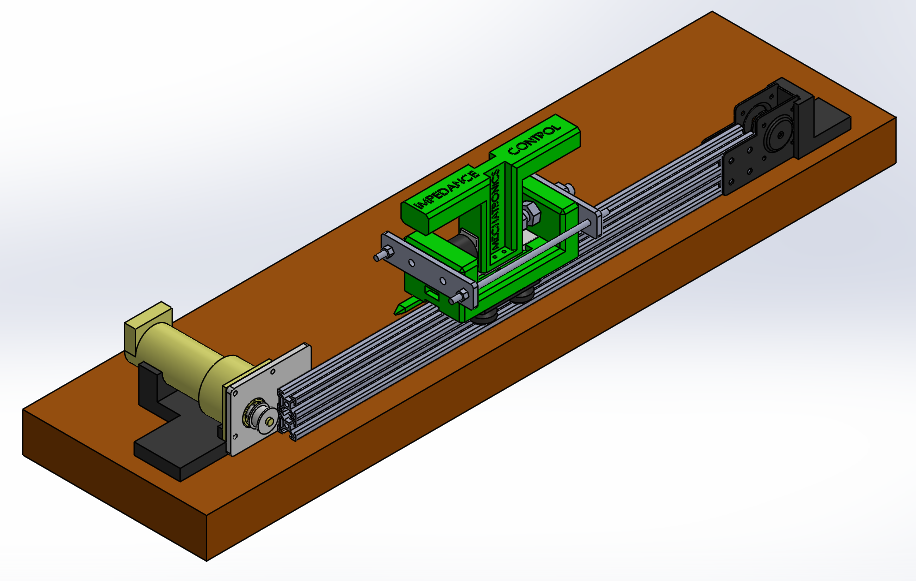
\includegraphics[width=0.85\columnwidth]{Images/Isometric_Full_View}
	\caption{Isometric CAD Model}
	\label{fig:Isometric_Full_View}
\end{figure}
\begin{figure}[h]
	\begin{center}
		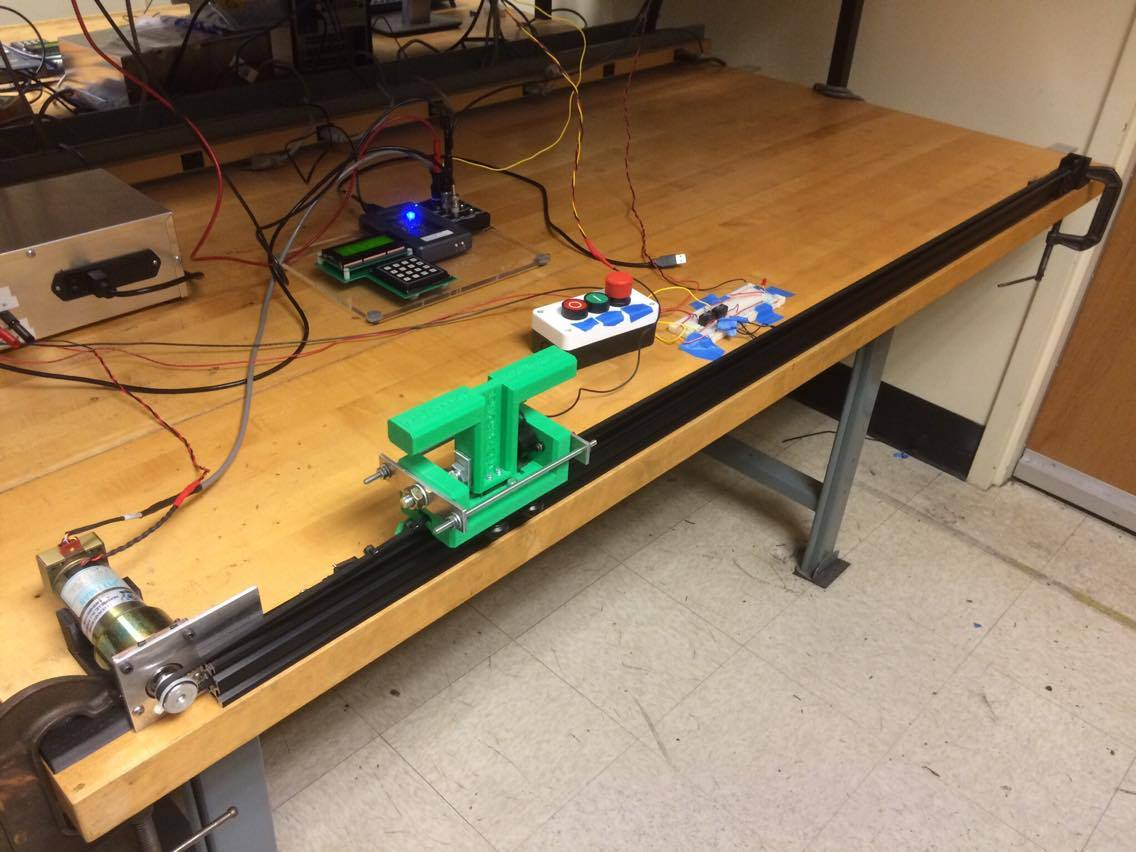
\includegraphics[width=0.85\columnwidth]{Images/Iso_Real_Full}
		\caption{Actual Prototype}
		\label{fig:Iso_Real_Full}
	\end{center}
\end{figure}
On the cart, there is a handle which is preloaded by an M10 Bolt onto a button load cell. Both the cart and handle are 3D printed. The user will apply a force to the handle sensed by the load cell which will be the input for our computer model and the cart should move accordingly based on the reference model. The challenge is to ensure that the force from the user is all transmitted to the load cell for an accurate input to the system model. One can imagine that as the handle is preloaded, there will more friction to overcome.

The first step to tackle this problem is to use small aluminum connecting plates on both sides of the handle that contact the load cell and preload. Since the handle was 3D printed PLA, the pressure from small contacting point of the load cell and the preload would only deform the soft PLA material. Adding the aluminum connecting plates allows for a stiffer area of contact and a consistent force to be applied to the load cell.

\begin{figure}[h]
	\centering
	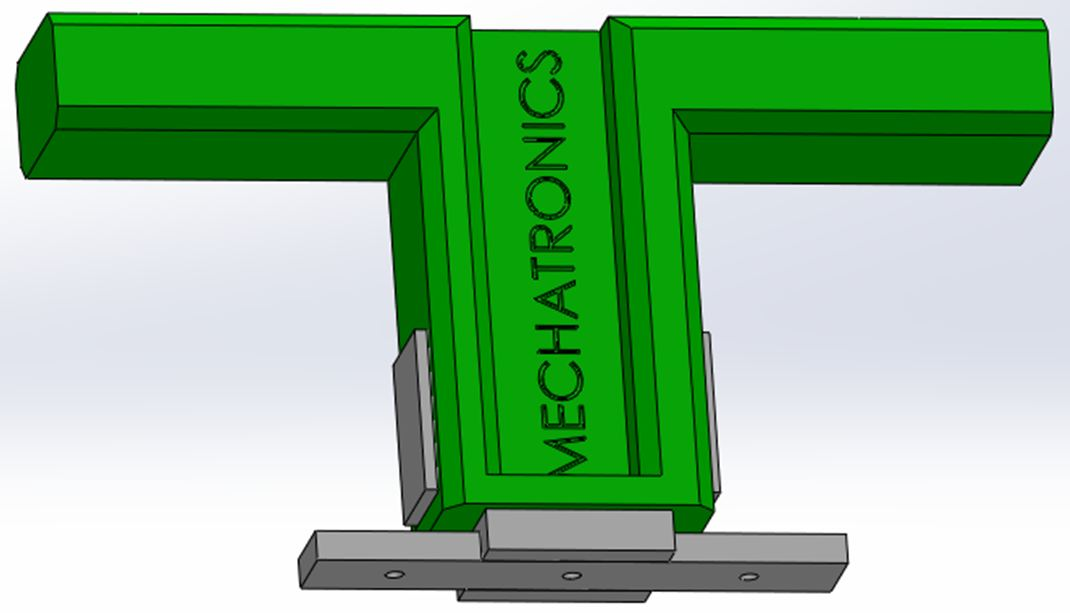
\includegraphics[width=0.8\columnwidth]{Images/Recirculating_Ball_Track}
	\caption{Handle on Recirculating Ball Track}
	\label{fig:Recirculating_Ball_Track}
\end{figure}

Taking a closer look, the handle is screwed on to a recirculating ball track as shown in Figure \ref{fig:Recirculating_Ball_Track}. The recirculating ball track is a key component to the mechanical design. Since the slider moves purely in a linear motion along the track, it minimizes friction and ensures that any force, even a torque, applied to the handle is completely transmitted to the load cell. Figure \ref{fig:Ball_Track_Cross_Section} shows a cross section of the handle and how it connects to the load cell, preload, ball track, and the rest of the cart. A labeled figure of the entire system is shown in Figure \ref{fig:Annotated_Front}.


\begin{figure}[h]
\centering
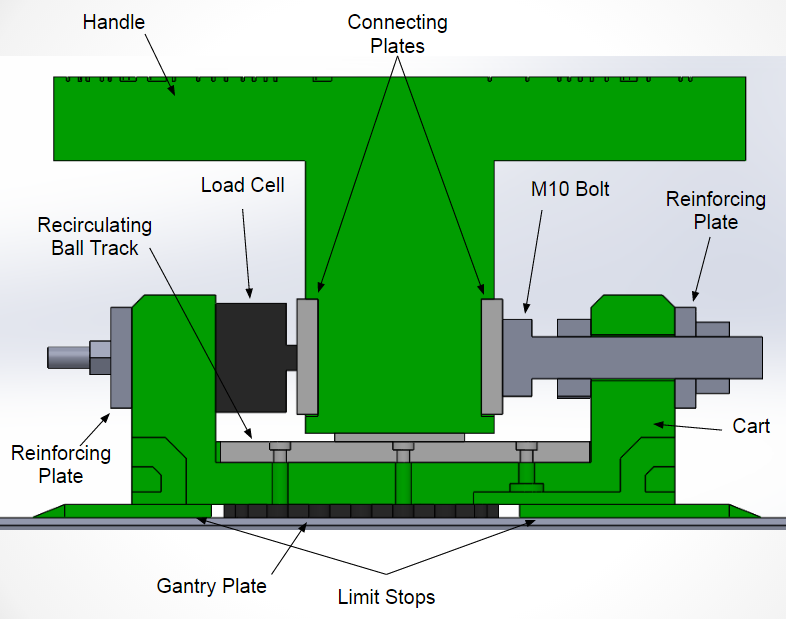
\includegraphics[width=0.8\columnwidth]{Images/Ball_Track_Cross_Section}
\caption{Cart Cross Section}
\label{fig:Ball_Track_Cross_Section}
\end{figure}

When designing the cart, PLA creep stiffness was not taken into account. Due to the rather elastic PLA material, a constant decrease in the preload would occur. This caused inconsistent force readings from the load cell. To counter this problem, two aluminum reinforcing plates were machined and held by threaded rods shown in Figure \ref{fig:Annotated_Iso}. This helped with the creep and overall cart stiffness, which gave much more accurate force readings from the load cell.
\begin{figure}[h]
	\centering
	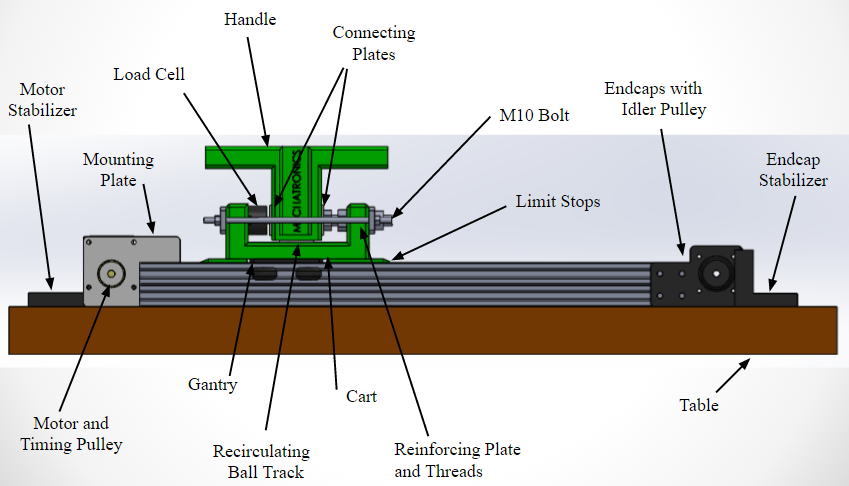
\includegraphics[width=1\linewidth]{Images/Annotated_Front}
	\caption{}
	\label{fig:Annotated_Front}
\end{figure}
\begin{figure}[h]	
\centering
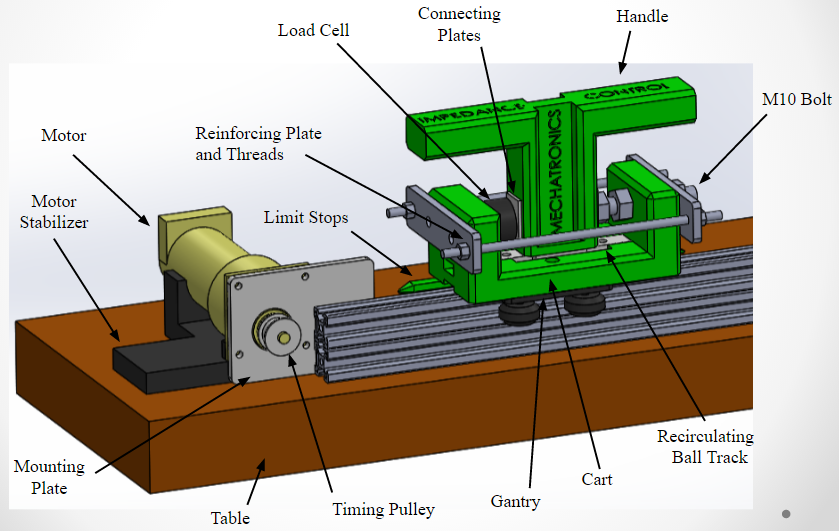
\includegraphics[width=1\linewidth]{Images/Annotated_Iso}
\caption{Labeled Isometric View}
\label{fig:Annotated_Iso}
\end{figure}
